\documentclass[12pt,aspectratio=169]{beamer}

\usetheme{metropolis}

\usefonttheme{professionalfonts}
\usepackage{graphicx}
\usepackage{tikz}
\usepackage{amsmath}
\usepackage{mathpazo}
\usepackage{xcolor,colortbl}
\usepackage{siunitx}
\usepackage[siunitx]{circuitikz} % to draw circuits!

\setmonofont{Ubuntu Mono}
\setlength{\parskip}{0pt}
\renewcommand{\baselinestretch}{1}

\sisetup{
  detect-all,
  number-math-rm=\mathnormal,
  per-mode=symbol
}

\title{Topic 13: Circuits Analysis}
\subtitle{Advanced Placement Physics}
\author[TML]{Dr.\ Timothy Leung}
\institute{Olympiads School, Toronto, ON, Canada}
\date{February 2020}


\newcommand{\pic}[2]{\includegraphics[width=#1\textwidth]{#2}}
\newcommand{\mb}[1]{\mathbf{#1}}
\newcommand{\eq}[2]{\vspace{#1}{\Large\begin{displaymath}#2\end{displaymath}}}


\begin{document}

\begin{frame}
  \maketitle
\end{frame}

\section{Current}

\begin{frame}{Current}
  We define conventional current as the rate at which positive charges flows
  through a wire, i.e.:

  \eq{-.3in}{\boxed{I=\frac{dQ}{dt}}}

  We can also think of the current as the flux of ``charge density'' flowing
  past a surface, i.e.:
  
  \eq{-.3in}{\boxed{I=\int\mb{J}\cdot d\mb{A}}}

  $d\mb{A}$ is defined the same way as Gauss's law, with its
  magnitude being the infinitesimal area $dA$ and the direction being the
  outward normal from the surface. This expression is especially important when
  dealing with plasma etc.
\end{frame}



\begin{frame}{Current}
  \begin{itemize}
  \item We now know that in a wire, instead of positive charges flowing in one
    direction, we have, in fact, electrons (negative charges) flowing in the
    opposite direction
  \item We are treating current as a scalar quantity, but later we will have to
    treat it as a vector
  \item As charges move through a conductor, they will lose potential energy
  \item How much energy it loses depends on the resistance of the material
  \end{itemize}
\end{frame}


\section{Resistors}

\begin{frame}{Resistivity}
  The resistivity of a material is proportional to the electric field and
  current density:

  \eq{-.3in}{
    \boxed{\mb{E}=\rho\mb{J}}
    \quad\quad\text{\large Scalar:}\quad
    \boxed{\rho=\left|\frac{E}{J}\right|}
  }
  \begin{center}
    \begin{tabular}{l|c|c}
      \rowcolor{pink}
      \textbf{Quantity} & \textbf{Symbol} & \textbf{SI Unit} \\ \hline
      Electric field & $\mb{E}$ & \si{\newton/\coulomb} \\
      Charge density & $\mb{J}$ & \si{\ampere/m^2} \\
      Resistivity & $\rho$ & \si{\ohm/\metre}
    \end{tabular}
  \end{center}
\end{frame}



\begin{frame}{Resistivity}

  \eq{-.05in}{
    \boxed{\mb{E}=\rho\mb{J}}
    \quad\quad\text{\large Scalar:}\quad
    \boxed{\rho=\left|\frac{E}{J}\right|}
  }
  \begin{itemize}
  \item In a conductor, because the electrons are free to move, the electric
    field tend to be very small, and the resistivity is low.
  \item In a dielectric (non conducting material), electrons cannot move
    easily--only polarize themselves--the electric field are generally strong,
    and the resistivity is higher.
  \end{itemize}
\end{frame}



\begin{frame}{Resistance of a Conductor}
  The resistance of a conductor is proportional to the resistivity $\rho$ and
  its length $L$, and inversely proportional to the cross-sectional area $A$:

  \eq{-.2in}{
    \boxed{R = \rho\frac{L}{A}}
  }
  \begin{center}
    \begin{tabular}{l|c|l}
      \rowcolor{pink}
      \textbf{Quantity} & \textbf{Symbol} & \textbf{SI Unit} \\ \hline
      Resistance           & $R$    & \si{\ohm} \\
      Resistivity          & $\rho$ & \si{\ohm.\metre} (ohm metres) \\
      Length of conductor  & $L$    & \si{\metre} (metres) \\
      Cross-sectional area & $A$    & \si{\metre^2} (square metres)
    \end{tabular}
  \end{center}
\end{frame}


\begin{frame}{Resistance of a Conductor}
  \eq{-.01in}{
    \boxed{R = \rho\frac{L}{A}}
  }

  \begin{columns}
    \column{0.5\textwidth}
    \begin{center}
      \begin{tabular}{c|c|c}
        \rowcolor{blue!50}
        {\color{white}Gauge} & 
        {\color{white}Diameter} & 
        {\color{white}$R/L$} \\
        \rowcolor{blue!50}
        & {\color{white}(\si{mm})} & 
        {\color{white}(\SI{e-3}{\ohm/m})}\\ \hline
        0  & \num{9.35} & \num{0.31} \\
        10 & \num{2.59} & \num{2.20} \\
        14 & \num{1.63} & \num{8.54} \\
        18 & \num{1.02} & \num{21.90} \\
        22 & \num{0.64} & \num{51.70} \\
      \end{tabular}
    \end{center}
    
    \column{.5\textwidth}
    \begin{center}
      \begin{tabular}{c|c}
        \rowcolor{blue!50}
        {\color{white} Material} & 
        {\color{white} Resistivity $\rho$ (\si{\ohm.m})}\\ \hline
        silver    & \num{1.6e-8} \\
        copper    & \num{1.7e-8} \\
        aluminum  & \num{2.7e-8} \\
        tungsten  & \num{5.6e-8} \\
        Nichrome  & \num{100e-8} \\
        carbon    & \num{3500e-8}\\
        germanium & \num{0.46} \\
        glass     & \num{e10} to \num{e14}\\
      \end{tabular}
    \end{center}
  \end{columns}
\end{frame}



\section{Ohm's Law}

\begin{frame}{Ohm's Law}
  The electric potential difference $V$ across a ``load'' (resistor) equals the
  product of the current $I$ through the load and the resistance $R$ of the
  load.

  \eq{-.2in}{
    \boxed{V=IR}
  }
  \begin{center}
    \begin{tabular}{l|c|c}
      \rowcolor{pink}
      \textbf{Quantity} & \textbf{Symbol} & \textbf{SI Unit} \\ \hline
      Potential difference & $V$    & \si{\volt} \\
      Current              & $I$    & \si{\ampere}\\
      Resistance           & $R$    & \si{\ohm}
    \end{tabular}
  \end{center}
  A resistor is considered ``ohmic'' if it obeys Ohm's law
\end{frame}


\begin{frame}{Power Dissipated by a Resistor}
  Power is the rate at which work $W$ is done, and from electrostatics, the
  change in electric potential energy $\Delta E_q$ (i.e.\ the work done!) is
  proportional to the amount of charge $q$ and the voltage $V$. This gives a
  very simple expression for power through a resistor:
  
  \eq{-.15in}{
    P=\frac{dW}{dt}=\frac{d(qV)}{dt}=\left(\frac{dq}{dt}\right)V
    \;\rightarrow\;\boxed{P=IV}
  }
  
  \begin{center}
    \begin{tabular}{l|c|c}
      \rowcolor{pink}
      \textbf{Quantity} & \textbf{Symbol} & \textbf{SI Unit} \\ \hline
      Power through a resistor    & $P$ & \si{\watt} \\
      Current through a resistor  & $I$ & \si{\ampere} \\
      Voltage across the resistor & $V$ & \si{\volt}
    \end{tabular}
  \end{center}
\end{frame}



\begin{frame}{Other Equations for Power}
  When we combine Ohm's Law ($V=IR$) with power equation, we get two additional
  expressions for power through a resistor:

  \eq{-.2in}{
    \boxed{P=\frac{V^2}{R}}\quad\boxed{P=I^2R}
  }
  \begin{center}
    \begin{tabular}{l|c|c}
      \rowcolor{pink}
      \textbf{Quantity} & \textbf{Symbol} & \textbf{SI Unit} \\ \hline
      Power      & $P$ & \si{\watt} \\
      Voltage    & $V$ & \si{\volt} \\
      Resistance & $R$ & \si{\ohm}  \\
      Current    & $I$ & \si{\ampere}
    \end{tabular}
  \end{center}
\end{frame}


\section{Kirchkoff's Laws}

\begin{frame}{Kirchkoff's Current Law}
  The electric current that flows into any junction in an electric circuit must
  be equal to the current which flows out.

  \vspace{.2in}
  \begin{columns}
    \column{.3\textwidth}
    \begin{center}
      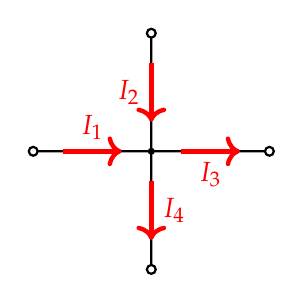
\begin{tikzpicture}[scale=1.5]
        \draw[thick](0,0) to[short,o-] (1,0) to[short,-o] (1,-1);
        \draw[thick](1,1) to[short,o-] (1,0) to[short,-o] (2,0);
        \draw[ultra thick,red,->](.25,0)--(.75,0) node[midway,above]{$I_1$};
        \draw[ultra thick,red,->](1,.75)--(1,.25) node[midway,left]{$I_2$};
        \draw[ultra thick,red,->](1.25,0)--(1.75,0) node[midway,below]{$I_3$};
        \draw[ultra thick,red,->](1,-.25)--(1,-.75) node[midway,right]{$I_4$};
        \fill[black](1,0) circle(0.03);
      \end{tikzpicture}
    \end{center}
    
    \column{.7\textwidth}
    e.g.\ if there are 4 paths to the junction at the center, with $I_1$ and
    $I_2$ going into the junction, and $I_3$ and $I_4$ coming out, then the
    current law says that

    \eq{-.3in}{
      I_1+I_2-I_3-I_4=0
    }
  \end{columns}

  \vspace{.2in}Basically, it means that there cannot be any accumulation of
  charges anywhere in the circuit. The law is a consequence of conservation of
  energy.
\end{frame}



\begin{frame}{Kirchkoff's Voltage Law}
  The voltage changes around any closed loop in the circuit must sum to zero,
  no matter what path you take through an electric circuit.

  \vspace{.1in}
  \begin{columns}
    \column{.3\textwidth}
    \begin{center}
      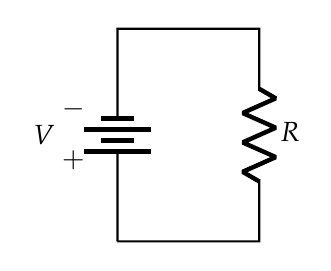
\begin{tikzpicture}[scale=1.8,american voltages]
        \draw[thick](0,0) to[battery=$V$] (0,1.5)--(1,1.5) to[R=$R$] (1,0)--(0,0);
      \end{tikzpicture}
    \end{center}
    \column{.7\textwidth}
    Assume that the current flows clockwise and we draw a clockwise loop, we
    get

    \eq{-.45in}{ V-V_R=0\;\;\rightarrow\;\; V-IR=0}

    \vspace{-.25in}If I incorrectly guess that $I$ flows counterclockwise, I
    will still have a similar expression

    \eq{-.45in}{-V_R-V=0\;\;\rightarrow\;\; -V-IR=0}
  \end{columns}

  \vspace{-.1in}When solving for $I$, we get a negative number, indicating
  that my guess was in the wrong direction.
\end{frame}



\section{Resistors in Circuits}

\begin{frame}{Resistors in Parallel}
  \begin{columns}
    \column{.32\textwidth}
    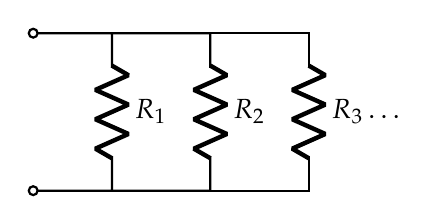
\begin{tikzpicture}
     \draw[thick] (0,2) to[short,o-] (1,2) to[R=$R_1$] (1,0) to[short,-o] (0,0);
     \draw[thick](1,2)  to[short] (2.25,2)to[R=$R_2$] (2.25,0)to[short] (1,0);
     \draw[thick](2.25,2)to[short](3.5,2) to[R=$R_3\ldots$] (3.5,0)
     to[short] (2.25,0);
    \end{tikzpicture}
    \column{.68\textwidth}
    From the current law, we know that the total current is the
    current through all the resistors, which we can rewrite in terms of voltage
    and resistance using Ohm's law:

    \vspace{-.3in}{\large
      \begin{displaymath}
        I=I_1+I_2+I_3\cdots=\frac{V_1}{R_1}+\frac{V_2}{R_2}+\frac{V_3}{R_3}\cdots
      \end{displaymath}
    }
    
    \vspace{-.2in}But since we also know that $V_1=V_2=V_3=\cdots=V$ from the
    voltage law, we can re-write as

    \eq{-.3in}{
      I=\frac{V}{R_\mathrm{eq}}=V\left(\frac{1}{R_1}+\frac{1}{R_2}+\frac{1}{R_3}
      \cdots\right)
    }
  \end{columns}
\end{frame}



\begin{frame}{Resistors in Parallel}{Equivalent Resistance}
  Through applying Ohm's Law and Kirchkoff's laws, we find the equivalent
  resistance of a parallel circuit, which we have known since Grade 9: The
  inverse of the equivalent resistance for resistors connected in parallel is
  the sum of the inverses of the individual resistances.

  \eq{-.2in}{
    \boxed{
      \frac{1}{R_p}
      =\frac{1}{R_1}+\frac{1}{R_2}+\cdots+\frac{1}{R_N}
    }
  }
  \begin{center}
    \begin{tabular}{l|c|c}
      \rowcolor{pink}
      \textbf{Quantity} & \textbf{Symbol} & \textbf{SI Unit} \\ \hline
      Equivalent resistance in parallel & $R_p$ & \si{\ohm} \\
      Resistance of individual loads    & $R_{1,2,3,\cdots,N}$ & \si{\ohm}
    \end{tabular}
  \end{center}
\end{frame}



\begin{frame}{Resistors in Series}
  \begin{center}
    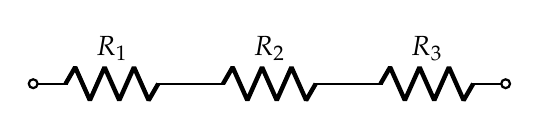
\begin{tikzpicture}
      \draw[thick](0,0) to[R=$R_1$,o-] (2,0) to[R=$R_2$] (4,0)
      to[R=$R_3$,-o] (6,0);
    \end{tikzpicture}
  \end{center}

  \vspace{.1in}The analysis for resistors in series is similar (but easier).
  From the current law, the current through each resistor is the same:

  \eq{-.2in}{I_1=I_2=I_3=\cdots=I}

  \vspace{-.15in}And the total voltage drop across all resistor is therefore:

  \eq{-.3in}{V=V_1+V_2+V_3+\cdot=I(R_1+R_2+R_3+\cdots)}
\end{frame}



\begin{frame}{Resistors in Series}{Equivalent Resistance}
  Again, through applying Ohm's Law and Kirchkoff's laws, we find that when
  resistors are connected in series: the equivalent resistance of loads is the
  sum of the resistances of the individual loads.
  
  \eq{-.2in}{
    \boxed{R_s=\sum_{i=1}^{N}R_i}
  }
  \begin{center}
    \begin{tabular}{l|c|c}
      \rowcolor{pink}
      \textbf{Quantity} & \textbf{Symbol} & \textbf{SI Unit} \\ \hline
      Equivalent resistance in series & $R_s$ & \si{\ohm} \\
      Resistance of individual loads & $R_{1,2,3,\cdots,N}$ & \si{\ohm}
    \end{tabular}
  \end{center}
\end{frame}


%\begin{frame}{Example Problem (Simple)}
%  A simple circuit analysis problem will involve one voltage source and
%  resistors connected, some in parallel, and some in series. Below is a typical
%  example:
%
%  \vspace{.2in}
%  \begin{columns}
%    \column{.4\textwidth}
%    \begin{tikzpicture}[scale=.8,american voltages]
%      \draw(0,0) to[R=2<\ohm>](0,2) to[battery=100<\volt>] (0,4) to[short]
%      (1,4) to [R=10<\ohm>] (3,4)--(3,4.5) to[R=40<\ohm>] (5,4.5)
%      to[short] (5,4) to[short] (5.5,4)--(5.5,0)--(0,0);
%      \draw(3,4)--(3,3.5) to[R,l_=10<\ohm>] (5,3.5)--(5,4);
%      \draw[dashed] (-1.8,0.25) rectangle(0.6,3.75);
%    \end{tikzpicture}
%    \column{.6\textwidth}
%    Two \SI{10}{\ohm} resistors and a \SI{40}{\ohm} resistor are connected as
%    shown to a \SI{100}{\volt} emf source with internal resistance
%    \SI{2}{\ohm}. How much power is dissipated by the \SI{40}{\ohm} resistor?
%    \begin{enumerate}[(A)]
%    \item\SI{160}{\watt}
%    \item\SI{40}{\watt}
%    \item\SI{400}{\watt}
%    \item\SI{5}{\watt}
%    \item\SI{500}{\watt}
%    \end{enumerate}
%  \end{columns}
%\end{frame}



\begin{frame}{Tips for Solving ``Simple'' Circuit Problems}
  \begin{enumerate}
  \item Identify groups of resistors that are in parallel or in series, and
    find their equivalent resistance.
  \item Gradually reduce the entire circuit to one voltage source and one
    resistor.
  \item Using Ohm's law, find the current out of the battery.
  \item Using Kirchkoff's laws, find the current through each of the resistors.
  \end{enumerate}
\end{frame}



\begin{frame}{Circuits Aren't Always Simple}
  Some of these problems require you to solve a system of linear equations.
  The following is a simple example with two voltage sources:
  \begin{center}
    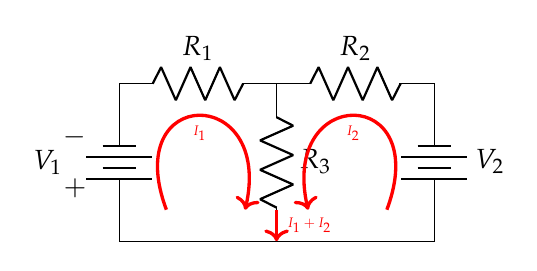
\begin{tikzpicture}[american voltages]
      \draw(0,0) to[battery=$V_1$](0,2) to[R=$R_1$](2,2) to[R=$R_3$](2,0)--(0,0);
      \draw(2,0)--(4,0) to[battery,l_=$V_2$](4,2) to[R,l_=$R_2$](2,2);
      \uncover<2->{
        \draw[very thick,red,->](2,0.4)--(2,0)
        node[midway,right]{\tiny $I_1+I_2$};
        \draw[very thick,red,->] (0.6,0.4)..controls (0,2) and (2,2)..(1.6,.4)
        node[midway,below]{\tiny $I_1$};
        \draw[very thick,red,->] (3.4,0.4)..controls (4,2) and (2,2)..(2.4,.4)
        node[midway,below]{\tiny $I_2$};
      }
    \end{tikzpicture}
  \end{center}
  \uncover<2->{
    In this case, we have to draw two loops of current.
  }
\end{frame}



\begin{frame}{A More Difficult Example}
  \begin{columns}
    \column{.4\textwidth}
    
    \vspace{-.3in}
    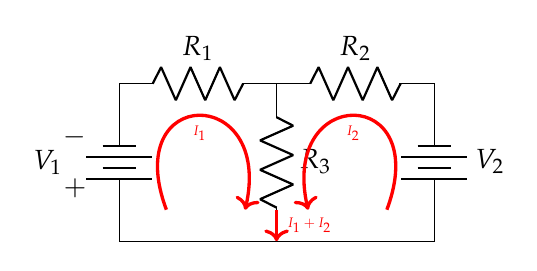
\begin{tikzpicture}[american voltages]
      \draw(0,0) to[battery=$V_1$](0,2) to[R=$R_1$](2,2)to[R=$R_3$](2,0)--(0,0);
      \draw(2,0)--(4,0) to[battery,l_=$V_2$](4,2) to[R,l_=$R_2$](2,2);
      \draw[very thick,red,->](2,0.4)--(2,0)
      node[midway,right]{\tiny $I_1+I_2$};
      \draw[very thick,red,->] (0.6,0.4)..controls (0,2) and (2,2)..(1.6,.4)
      node[midway,below]{\tiny $I_1$};
      \draw[very thick,red,->] (3.4,0.4)..controls (4,2) and (2,2)..(2.4,.4)
      node[midway,below]{\tiny $I_2$};
    \end{tikzpicture}
    \column{.6\textwidth}
    We split the circuit into two loops, and apply Kirchkoff's voltage in both:

    \vspace{-.4in}{\Large
      \begin{align*}
        V_1-I_1R_1-(I_1+I_2)R_3&=0\\
        V_2-I_2R_2-(I_1+I_2)R_3&=0
      \end{align*}
    }
  \end{columns}

  \vspace{-.1in}Two equations, two unknowns ($I_1$ and $I_2$). We can subtract
  (2) from (1), then solve for $I_1$ and $I_2$:

  \eq{-.4in}{
    I_1=\frac{V_1-I_2R_3}{R_1+R_3}
    \quad\quad
    I_2=
    \frac{\left[V_2-\frac{(V_1-V_2)R_3}{R_1}\right]}
         {\left[R_2+\frac{(R_1+R_2)R_3}{R_1}\right]}
  }

  (Try this at home as an exercise.)
\end{frame}


\begin{frame}{This is As Difficult As It'll Get}
  \framesubtitle{And This Is Your Homework}
  \begin{columns}
    \column{.45\textwidth}
    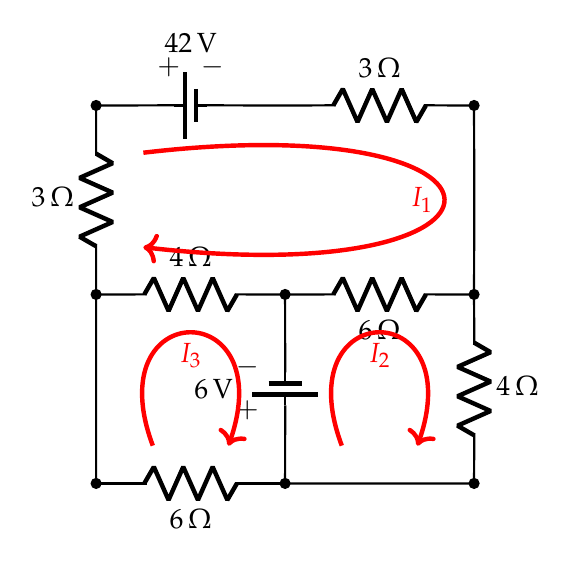
\begin{tikzpicture}[american voltages,scale=1.2]
      \draw[thick](0,0) to[short,*-](0,2) to[R=3<\ohm>,*-] (0,4)
      to[battery1=42<\volt>,*-](2,4) to[R=3<\ohm>] (4,4) to[short,*-](4,2)
      to[R=4<\ohm>,*-](4,0) to[short,*-](2,0) to[battery1=6<\volt>,*-](2,2)
      to[R,l_=4<\ohm>,*-](0,2);
      \draw[thick](0,0) to[R,l_=6<\ohm>](2,0);
      \draw[thick](2,2) to[R,l_=6<\ohm>](4,2);
      \uncover<2->{
        \draw[ultra thick,red,->]
        (.5,3.5)..controls(4.75,4)and(4.75,2)..(.5,2.5)
        node[midway,left]{$I_1$};
        \draw[ultra thick,red,->] (0.6,0.4)..controls (0,2) and (2,2)..(1.4,.4)
        node[midway,below]{$I_3$};
        \draw[ultra thick,red,->] (2.6,0.4)..controls (2,2) and (4,2)..(3.4,.4)
        node[midway,below]{$I_2$};
      }
    \end{tikzpicture}

    
    \column{.55\textwidth}
    \begin{itemize}
    \item To solve this problem, we define a few ``loops'' around the circuit:
      one on top, one on bottom left, and one on bottom right.
    \item<2-> Apply the voltage law in the loops. For example, in the
      lower left:

      \eq{-.5in}{
        4(I_1-I_3)-6-6I_3=0
      }      
    \item<2->\vspace{-.1in} Solve the linear system to find the current. If the
      current that you worked out is negative, it means that you have the
      direction wrong.
    \end{itemize}
  \end{columns}
\end{frame}



\section{Capacitors in Circuit}

\begin{frame}{Capacitors in Parallel}
  \begin{center}
    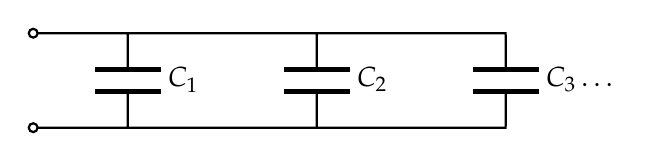
\begin{tikzpicture}[scale=1.2]
      \draw[thick](0,1)to[short,o-](1,1) to[C=$C_1$] (1,0)to[short,-o](0,0);
      \draw[thick](1,1)--(3,1) to[C=$C_2$]       (3,0)--(1,0);
      \draw[thick](3,1)--(5,1) to[C=$C_3\ldots$] (5,0)--(3,0);
    \end{tikzpicture}
  \end{center}
  From the voltage law, we know that the voltage across all the capacitors are
  the same, i.e.\ $V_1=V_2=V_3-\cdots=V$. We can express the total charge
  $Q_\mathrm{tot}$ stored across all the capacitors in terms
  of capacitance and this
  common voltage $V$: 

  \eq{-.3in}{
    Q_\mathrm{tot}=Q_1+Q_2+Q_3+\cdots=C_1V+C_2V+C_3V+\cdots
  }
  
  \vspace{-.1in}Factoring out $V$ from each term gives us the equivalent
  capacitance:

  \eq{-.2in}{
    \boxed{C_p=\sum_i C_i}
  }
\end{frame}


\begin{frame}{Capacitors in Series}
  Likewise, we can do a similar analysis to capacitors connected in series.
  \begin{center}
    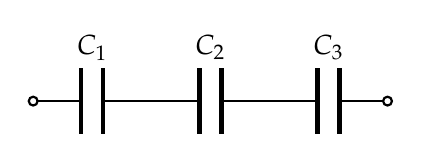
\begin{tikzpicture}[scale=1.2]
      \draw[thick](0,0) to[C=$C_1$,o-] (1.25,0) to[C=$C_2$] (2.5,0)
      to[C=$C_3$,-o] (3.75,0);
    \end{tikzpicture}
  \end{center}
  The total voltage across these capacitors are the sum of the voltages across
  each of them, i.e.\ $V_\mathrm{tot}=V_1+V_2+V_3+\cdots$
  
  \vspace{.1in}We recognize that the charge stored on all the capacitors must
  be the same! We can then write the total voltage in terms of capacitance and
  charge:

  \eq{-.25in}{
    V_\mathrm{tot}=\frac{Q}{C_1}+\frac{Q}{C_2}+\frac{Q}{C_3}+\cdots
  }
\end{frame}




\begin{frame}{Capacitors in Series}{Equivalent Capacitance}
  The inverse of the equivalent capacitance for $N$ capacitors connected in
  series is the sum of the inverses of the individual capacitance.

  \eq{-.2in}{
    \boxed{ \frac{1}{C_s}=\sum_i\frac{1}{C_i} }
  }
  
  Make sure we don't confuse ourselves with resistors.
\end{frame}



\begin{frame}{How Do We Know That Charges Are The Same?}
  It's simple to show that the charges across all the capacitors are the same
  \begin{center}
    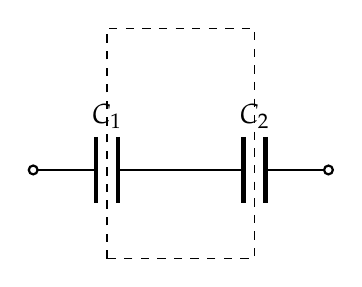
\begin{tikzpicture}[scale=1.5]
      \draw[thick](0,0) to[C=$C_1$,o-] (1.25,0) to[C=$C_2$,-o] (2.5,0);
      \draw[dashed](0.625,-.75) rectangle (1.875,1.2);
    \end{tikzpicture}
  \end{center}
  The capacitor plates and the wire connecting them are really one piece of
  conductor. There is nowhere for the charges to leave the conductor, therefore
  when charges are accumulating on $C_1$, $C_2$ must also have the same charge
  because of conservation of charges.
\end{frame}



\section{R-C Circuits}

\begin{frame}{Circuits with Resistors and Capacitors}
  Now that we have seen how resistors and capacitors behave in a circuit, we
  can look into combining them in to an ``R-C circuit''.
  \begin{center}
    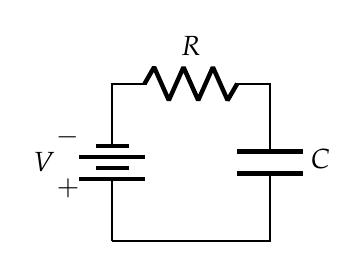
\begin{tikzpicture}[american voltages]
      \draw[thick](0,0)
      to[battery=$V$] (0,2)
      to[R=$R$] (2,2)
      to[C=$C$] (2,0)--(0,0);
    \end{tikzpicture}
  \end{center}
  The simplest form is a resistor and capacitor connected in series, and
  then connect to a voltage source. Because of the nature of capacitors, the
  current through the circuit will not be steady as were the case with only
  resistors.
\end{frame}



\begin{frame}{Discharging a Capacitor}
  We start the analysis with something even simpler. There is no voltage source,
  and the capacitor is already charged to $V_c=Q_\mathrm{tot}/C$. What happens
  when the current begin to flow?
  \begin{columns}
    \column{.3\textwidth}
    \begin{center}
      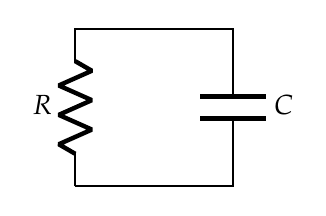
\begin{tikzpicture}
        \draw[thick](0,0) to[R=$R$] (0,2)--(2,2) to[C=$C$] (2,0)--(0,0);
      \end{tikzpicture}
    \end{center}
    
    \column{.7\textwidth}
    As current starts to flow, the charge on the capacitor decrease. Over time
    the current decreases, until the capacitor is fully discharged, and current
    stops flowing.
  \end{columns}

  \vspace{.15in}Apply the voltage law for the circuit, and substitute
  the definition of current $I=dQ/dt$ and the voltage across a capacitor
  $V_c=Q/C$:

  \eq{-.15in}{V_c-IR=0\quad\rightarrow\quad -\frac{Q}{C}-R\frac{dQ}{dt}=0}
\end{frame}


\begin{frame}{Discharging a Capacitor}
  Separating the $Q$ terms on the left side of the equation, and leaving
  everything else on the right side, we get:

  \eq{-.2in}{
    \frac{dQ}{Q}=\frac{-dt}{RC}
  }

  which we can now integrate and ``exponentiate'':

  \eq{-.15in}{
    \int\frac{dQ}{Q}=\int\frac{-dt}{RC}
    \;\rightarrow\;
    \ln Q=\frac{-t}{RC} + K
    \;\rightarrow\;
    Q=e^Ke^{-t/RC}
  }

  The constant of integration $K$ is the initial charge on the capacitor
  $Q_\mathrm{tot}$:

  \eq{-.2in}{
    e^K=Q_\mathrm{tot}
  }
\end{frame}



\begin{frame}{Discharging a Capacitor}
  The expression of charge across the capacitor is time-dependent:

  \eq{-.15in}{\boxed{Q(t)=Q_0e^{-t/\tau}}}

  \vspace{-.1in}where $Q_0=Q_\mathrm{tot}$ is the initial charge on the
  capacitor, and $\tau=RC$ is called the \textbf{time constant}. Taking the
  time derivative of $Q(t)$ gives us the current through the circuit:

  \eq{-.15in}{
    \boxed{I(t)=\frac{dQ}{dt}=I_0e^{-t/\tau}}
  }

  where the initially current at $t=0$ is given by
  $I_0=Q_\mathrm{tot}/\tau=Q_\mathrm{tot}/RC$.
\end{frame}



\begin{frame}{Charging a Capacitor}
  \vspace{.2in}
  \begin{columns}
    \column{.3\textwidth}
    \vspace{-.25in}
    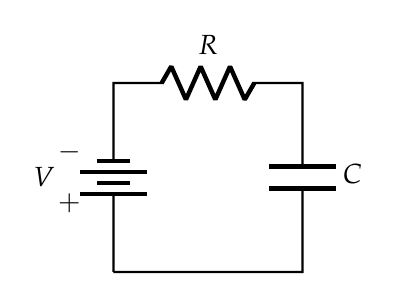
\begin{tikzpicture}[american voltages,scale=1.2]
      \draw[thick](0,0)
      to[battery=$V$] (0,2)
      to[R=$R$] (2,2)
      to[C=$C$] (2,0)--(0,0);
    \end{tikzpicture}
    
    \column{.7\textwidth}
    In charging up the capacitor, we go back to our original circuit, and apply
    the voltage law, then substitute the expression for current and voltage
    across the capacitor:

    \eq{-.15in}{
      V-R\frac{dQ}{dt}-\frac{Q}{C}=0
    }
  \end{columns}

  Again, separating variables, and integrating, we get:

  \eq{-.2in}{
    \int\frac{dQ}{CV-Q}=\int\frac{-dt}{RC}
    \;\;\rightarrow\;\;\ln(CV-Q)=\frac{-t}{RC}+K
  }
 \end{frame}



\begin{frame}{Charging a Capacitor}
  ``Exponentiating'' both sides, we have
  
  \eq{-.2in}{CV-Q=e^Ke^{-t/RC}}

  To find the constant of integration $K$, we note that at $t=0$, the charge
  across the capacitor is $0$, and we get

  \eq{-.2in}{e^K=CV=Q_\mathrm{tot}}

  which is the charge stored in the capacitor at the end. Substitute this back
  into the equation:

  \eq{-.2in}{
    \boxed{Q(t)=Q_\mathrm{tot}(1-e^{-t/RC})}
  }
\end{frame}




\begin{frame}{Capacitors}

  \eq{-.15in}{\boxed{Q(t)=Q_\mathrm{tot}(1-e^{-t/\tau})}}

  \vspace{-.1in}Charging a capacitor has the same time constant $\tau=RC$ as
  during discharge. We can also differentiate to find the current through the
  circuit; it is identical to the equation for discharge:

  \eq{-.2in}{
    \boxed{I(t)=\frac{dQ}{dt}=I_0e^{-t/\tau}}
  }

  where the initial current is given by $I_o=Q_\mathrm{tot}/\tau=V/R$. This
  makes sense because $V_C(t=0)=0$, and all of the energy must be dissipated
  through the resistor. Similarly at $I(t=\infty)=0$.
\end{frame}



\begin{frame}{Two Small Notes}
  \begin{enumerate}
  \item When a capacitor is uncharged, there is no voltage across the plate,
    it acts like a short circuit.
  \item When a capacitor is charged, there is a voltage across it, but no
    current flows \emph{through} it. Effectively it acts like an open circuit.
  \end{enumerate}
\end{frame}



\begin{frame}{A Slightly More Difficult Problem}
  \begin{center}
    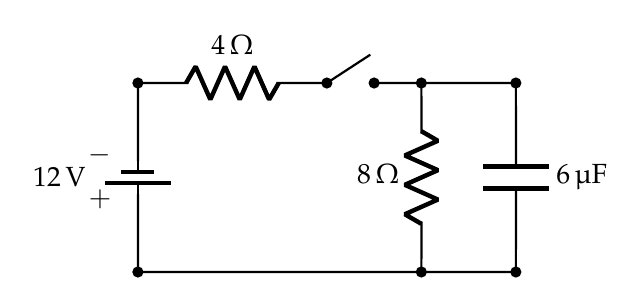
\begin{tikzpicture}[scale=1.2,american voltages]
      \draw[thick] (0,0) to[battery1=12<\volt>,*-*] (0,2) to[R=4<\ohm>] (2,2)
      to[short,*-](2.46,2.3);
      \draw[thick](2.5,2) to[short,*-*] (3,2) to[short,-*] (4,2)
      to[C=6<\micro\farad>,-*] (4,0)--(0,0);
      \draw[thick] (3,0) to[R=8<\ohm>,*-] (3,2);
    \end{tikzpicture}
  \end{center}
  \textbf{Example:} The capacitor in the circuit is initially uncharged. Find
  the current through the battery
  \begin{enumerate}
  \item Immediately after the switch is closed
  \item A long time after the switch is closed
  \end{enumerate}
\end{frame}


\section{LR Circuits}

\begin{frame}{Circuits with Inductors}
  \begin{itemize}
  \item Coils and solenoids in circuits are known as ``inductors'' and have
    large self inductance $L$
  \item Self inductance prevents currents rising and falling instantaneously
  \item A basic circuit containing a resistor and an inductor is called an
    \textbf{\emph{LR} circuit}:
    \begin{center}
      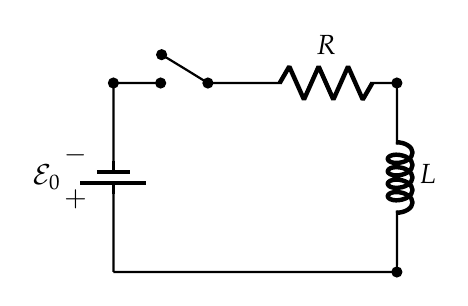
\begin{tikzpicture}[american voltages,scale=1.2]
        \draw[thick](0,0) to[battery1=$\mathcal{E}_0$,-*] (0,2)
        to[short,-*](0.5,2);
        \draw[thick](0.51,2.3) to[short,*-*](1,2)--(1.5,2) to [R=$R$,-*] (3,2)
        to [L=$L$,-*] (3,0)--(0,0);
      \end{tikzpicture}
    \end{center}
  \end{itemize}
\end{frame}

\begin{frame}
  \frametitle{Analyzing LR Circuits}
  \begin{columns}
    \column{.35\textwidth}
    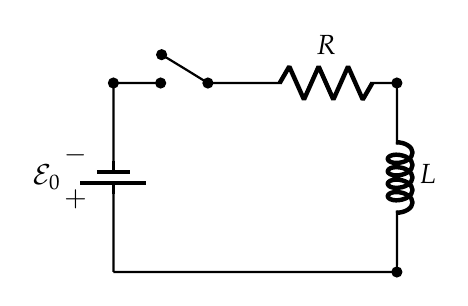
\begin{tikzpicture}[american voltages,scale=1.2]
      \draw[thick](0,0) to[battery1=$\mathcal{E}_0$,-*] (0,2)
      to[short,-*](0.5,2);
      \draw[thick](0.51,2.3) to[short,*-*](1,2)--(1.5,2) to [R=$R$,-*] (3,2)
      to [L=$L$,-*] (3,0)--(0,0);
    \end{tikzpicture}

    \column{.65\textwidth}
    Applying Kirchkoff's voltage law:

    \eq{-.2in}{\mathcal{E}_0-IR-L\frac{dI}{dt}=0}

    \vspace{-.1in}We follow the same procedure as charging a capacitor to find
    the time dependent current:

    \eq{-.2in}{I=\frac{\mathcal{E}_0}{R}\left(1-e^{-Rt/L}\right)}

    \vspace{-.15in} The time constant for an $LR$ circuit is
    
    \eq{-.2in}{\tau=\frac{L}{R}}
  \end{columns}
\end{frame}




%\begin{frame}
%  \frametitle{Magnetic Energy}
%  Just as a capacitor stores energy in its electric field, an inductor coil
%  carrying a current $I$ stores energy in its magnetic field, given by:
%
%  \eq{-.2in}{
%    \boxed{U_m=\frac{1}{2}LI^2}
%  }
%
%  We can also define a \textbf{magnetic energy density}:
%
%  \eq{-.2in}{
%    \boxed{\eta_m=\frac{B^2}{2\mu_0}}
%  }
%\end{frame}


\section{LC Circuit}

\begin{frame}{LC Circuit}
  The final type of circuit in AP Physics is the LC circuit. In its simplest
  form, the circuit has an inductor and capacitor connected in series:
  \begin{center}
    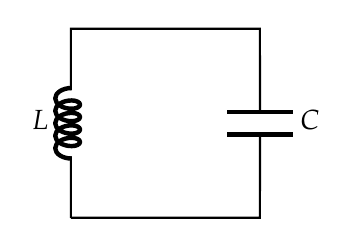
\begin{tikzpicture}[american voltages,scale=1.2]
      \draw[thick](0,0) to[L=$L$] (0,2)--(2,2) to[C=$C$] (2,0)--(0,0);
    \end{tikzpicture}
  \end{center}
  We apply the Kirchkoff's voltage law:
  
  \eq{-.2in}{
    -V_L-V_C=0
    \quad\rightarrow\quad
    L\frac{dI}{dt}+\frac{Q}{C}=0
  }
\end{frame}

\begin{frame}{LC Circuits}
  Since both terms are continuously differentiable, we can differentiate both
  sides of the equation, which gives:

  \eq{-.2in}{
    L\frac{d^2I}{dt^2}+\frac{1}{C}\underbrace{\frac{dQ}{dt}}_I=0
  }

  In fact, the above equation a second-order ordinary differential equation
  with constant coefficients. The solution to such an eqauation is the simple
  harmonic motion.

  \eq{-.2in}{
    \frac{d^2I}{dt^2}+\frac{1}{LC}I=0
  }


\end{frame}


\begin{frame}
  \frametitle{LC Circuit}
  The current inside of an LC circuit is given by:

  \eq{-.2in}{
    I(t)=I_0\sin(\omega t + \varphi)\quad\text{where}\quad
    \omega=\frac{1}{\sqrt{LC}}
  }
\end{frame}
\end{document}
